
%(BEGIN_QUESTION)
% Copyright 2014, Tony R. Kuphaldt, released under the Creative Commons Attribution License (v 1.0)
% This means you may do almost anything with this work of mine, so long as you give me proper credit

Industrial {\it control power transformers} are used to step down 480 or 240 volts to a level more acceptable for relay control circuitry: usually 120 volts.  Some control power transformers are built with multiple primary windings, to facilitate connection to either a 480 volt or 240 volt AC power source:

$$
\includegraphics[width=15.5cm]{i01259x01.eps}$$

Such transformers are usually advertised as having ``240 $\times$ 480'' primary windings, the ``$\times$'' symbol representing two independent windings with four connection points (H1 through H4).

Show the connections on the four ``H'' terminals necessary for 240 volt operation, and also for 480 volt operation, on the following illustrations:

$$\includegraphics[width=15.5cm]{i01259x02.eps}$$

\underbar{file i01259}
%(END_QUESTION)





%(BEGIN_ANSWER)

$$\includegraphics[width=15.5cm]{i01259x03.eps}$$

%(END_ANSWER)





%(BEGIN_NOTES)

This type of transformer is {\it very} common in industrial control systems.  Discuss with your students why the primary winding terminals are arranged as they are (H1-H3-H2-H4), to facilitate near-terminal jumpering with metal clips.

%INDEX% Electronics review: transformer ratios

%(END_NOTES)


